% This text is proprietary.
% It's a part of presentation made by myself.
% It may not used commercial.
% The noncommercial use such as private and study is free
% Sep. 2005 
% Author: Sascha Frank 
% University Freiburg 
% www.informatik.uni-freiburg.de/~frank/
% additional use of \usepackage{beamerthemesplit}
\documentclass{beamer}
\usepackage[utf8]{inputenc}
\usepackage[T2A]{fontenc} % кодировка шрифта
\usepackage[english,russian]{babel} % язык документа
\usepackage{beamerthemesplit}
\usepackage{graphicx}

\theoremstyle{plain}
\newtheorem{thm}{Теорема}[section]

\usetheme{Frankfurt}
\usecolortheme{orchid}


\usepackage{beamerthemesplit} % new 
\begin{document}
\title{Веб-приложение "BeeFat"} 
\author{Васильев Павел, Иудинов Михаил, Евтушенко Дмитрий}



\date{7 января 2024 г.}

\frame{\titlepage}

\section{Роли в команде} 
\frame{ 
\frametitle{Роли в  команде}


\begin{columns}
        \begin{column}{0.2\textwidth}
        	Михаил Иудинов: backend-developer
            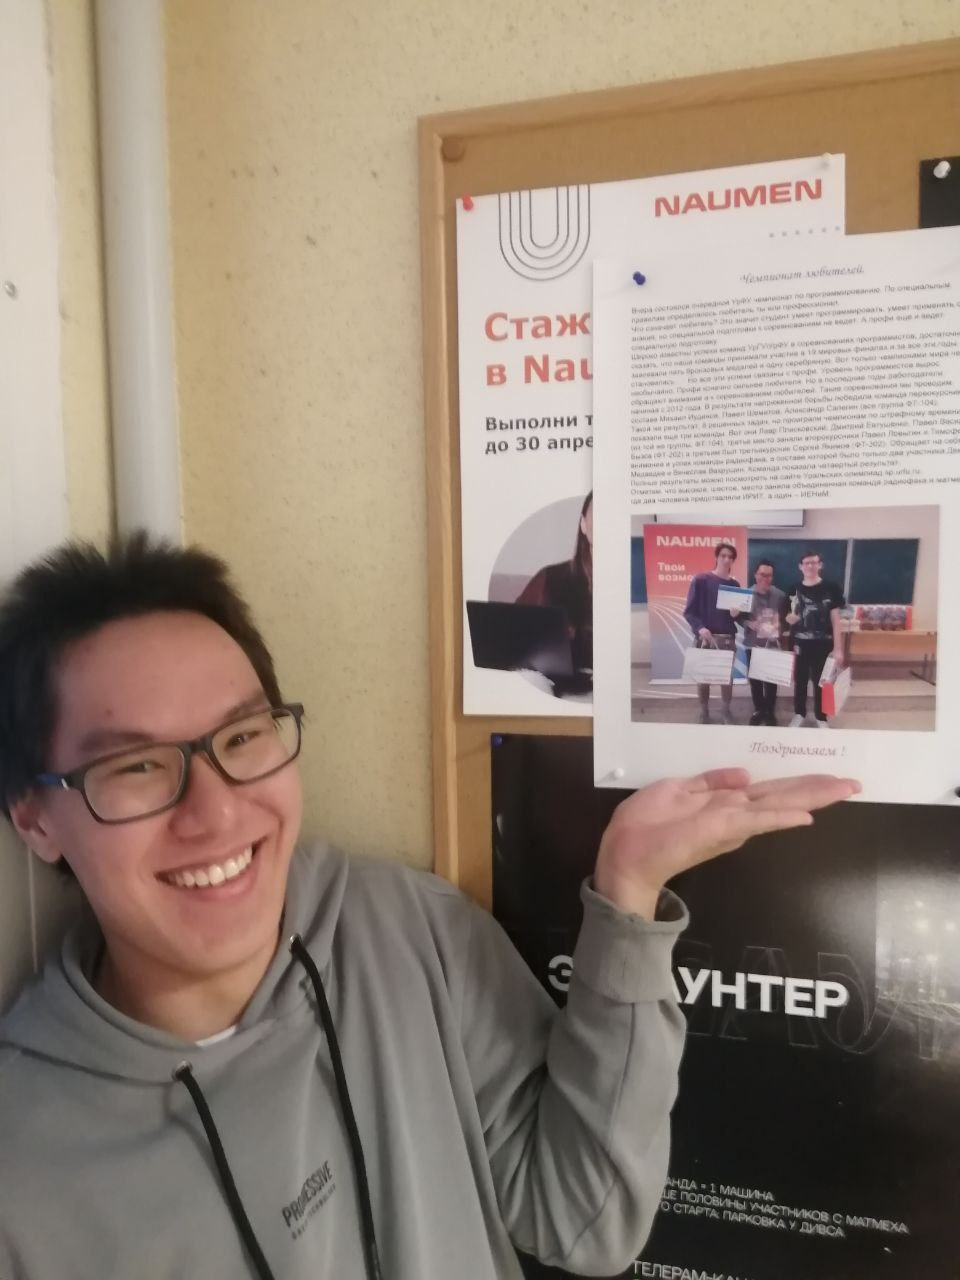
\includegraphics[width=3cm]{images/mi.jpg}
        \end{column}

        \begin{column}{0.2\textwidth}
        	Васильев Павел: fullstack-developer
            
\includegraphics[width=3cm]{images/pv.jpg}
        \end{column}
            
        \begin{column}{0.2\textwidth}
        	Евтушенко Дмитрий: product-manager
            
\includegraphics[width=3cm]{images/de.jpg}
        \end{column}
\end{columns}
}

\section{Проблема} 
\frame{ 

\frametitle{Проблема}

\begin{block}{Проблема}
Люди, которые хотят набрать массу, теряются в огромном количестве ресурсов по теме и тратят много времени на составление плана питания.
\end{block}

}


\section{Решение} 
\frame{ 

\frametitle{Решение}
\begin{block}{Решение}
    Наше приложение предлагает сбалансированный трек питания, направленный на набор массы. Таким образом, время составления рациона минимизируется.
\end{block}
}


\frame{ 
\frametitle{Скриншоты приложения}
"BeeFat" сразу предлагает сбалансированный рацион, нужны лишь параметры тела
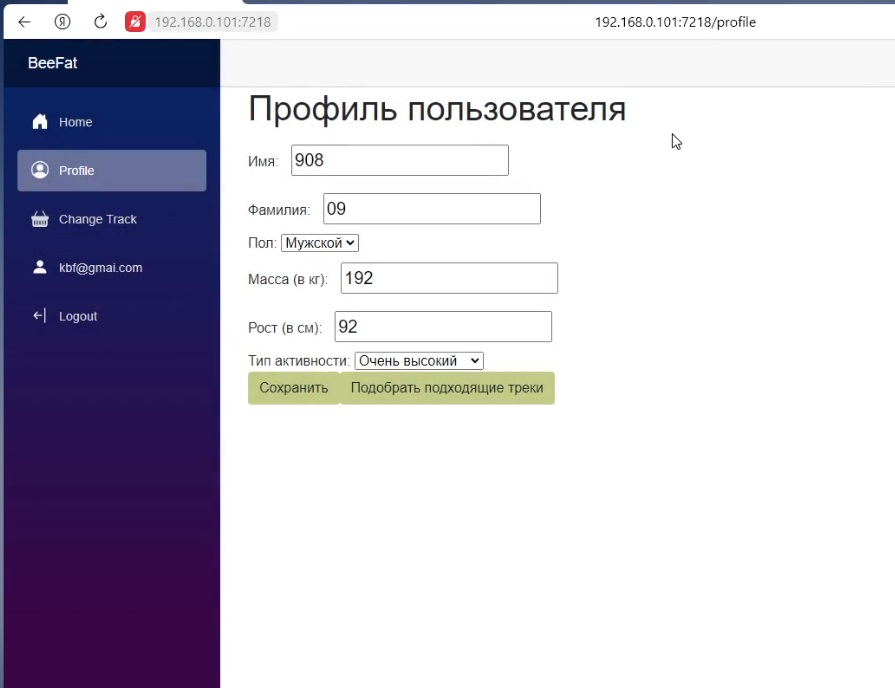
\includegraphics[width=10cm]{images/screenshot7.jpg}
}

\frame{ 
\frametitle{Скриншоты приложения}
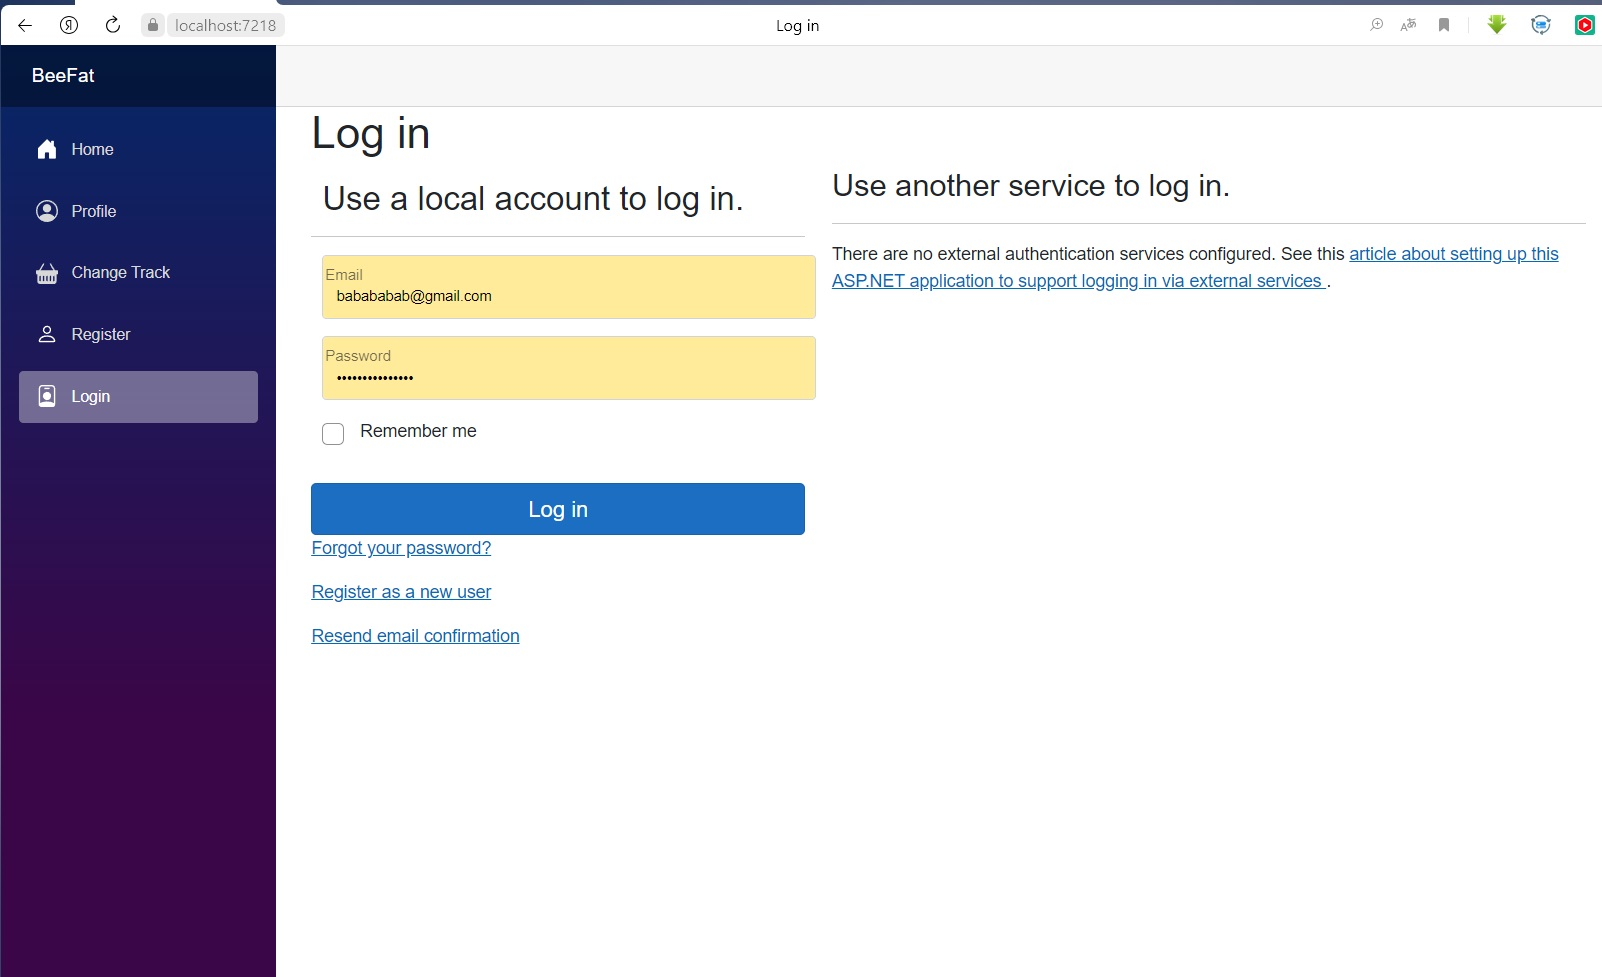
\includegraphics[width=10cm]{images/screenshot1.jpg}
}

\frame{ 
\frametitle{Скриншоты приложения}
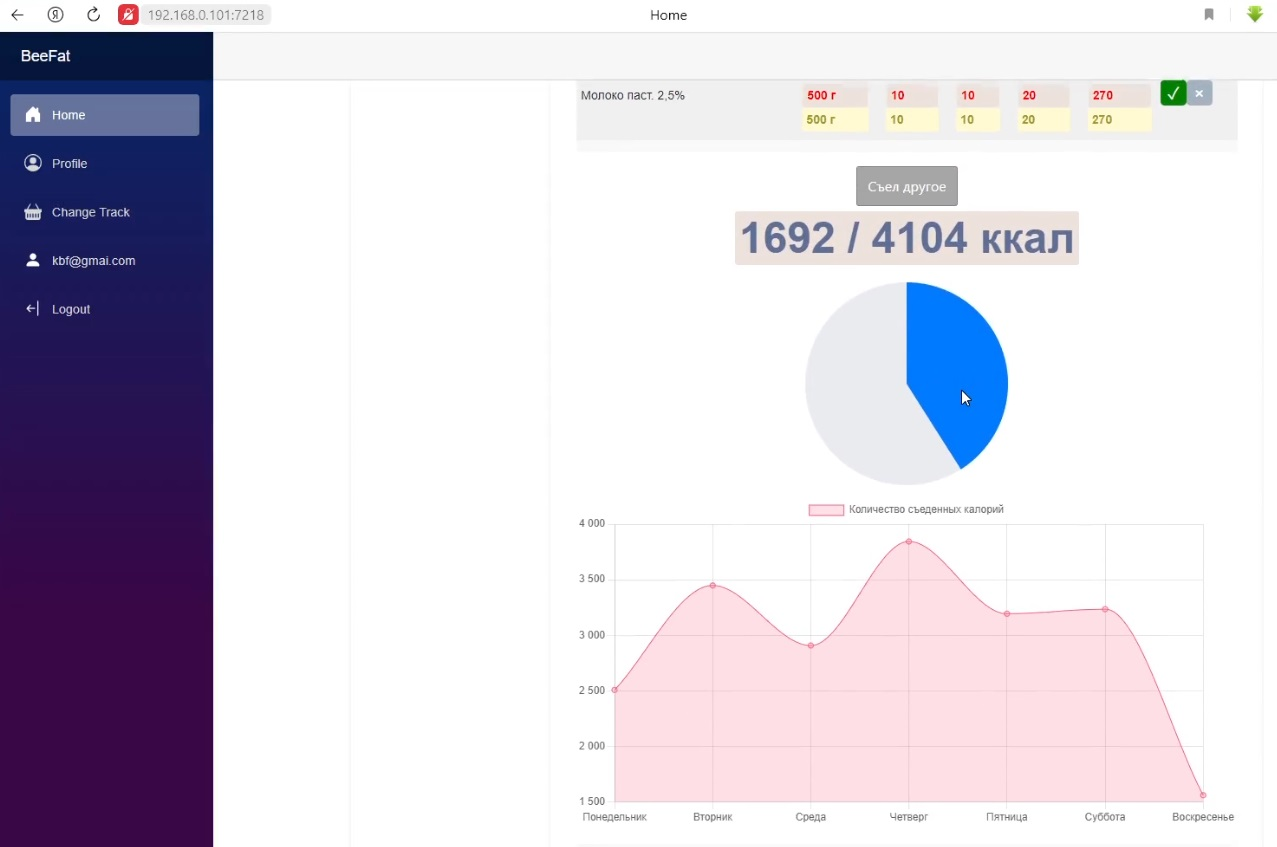
\includegraphics[width=10cm]{images/screenshot3.jpg}
}

\frame{ 
\frametitle{Скриншоты приложения}
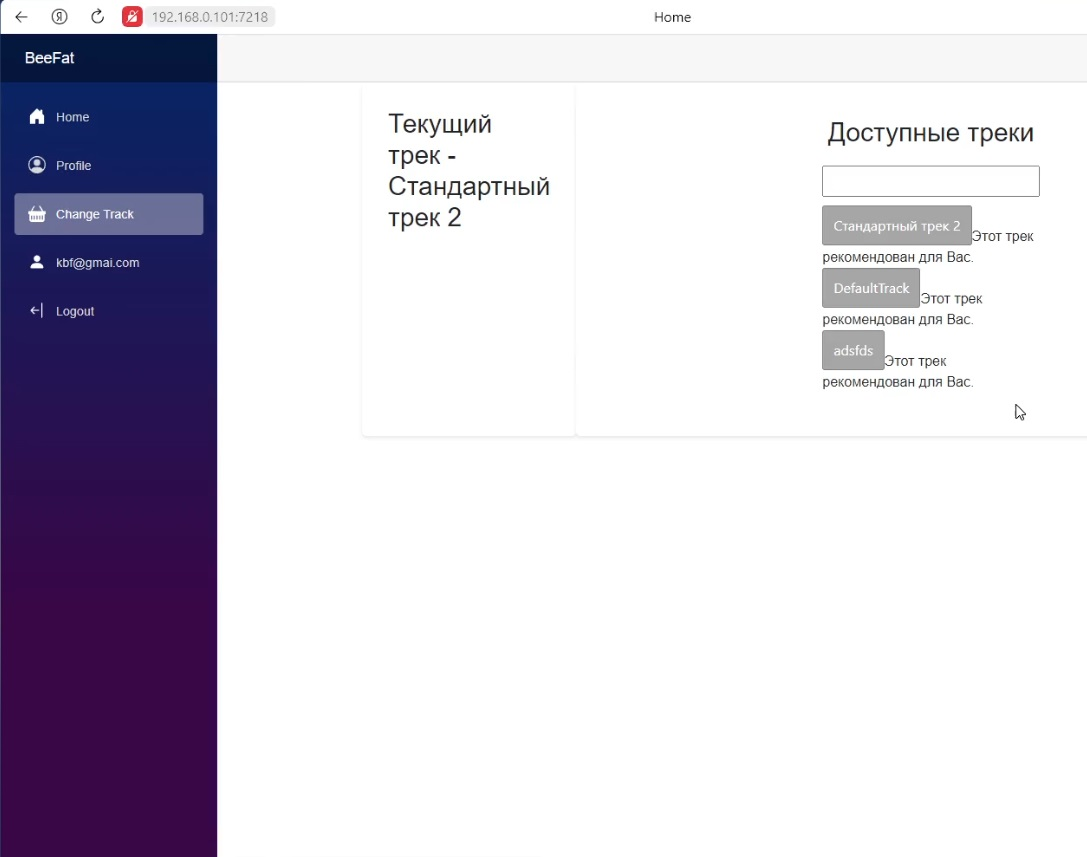
\includegraphics[width=10cm]{images/screenshot4.jpg}
}

\frame{ 
\frametitle{Скриншоты приложения}
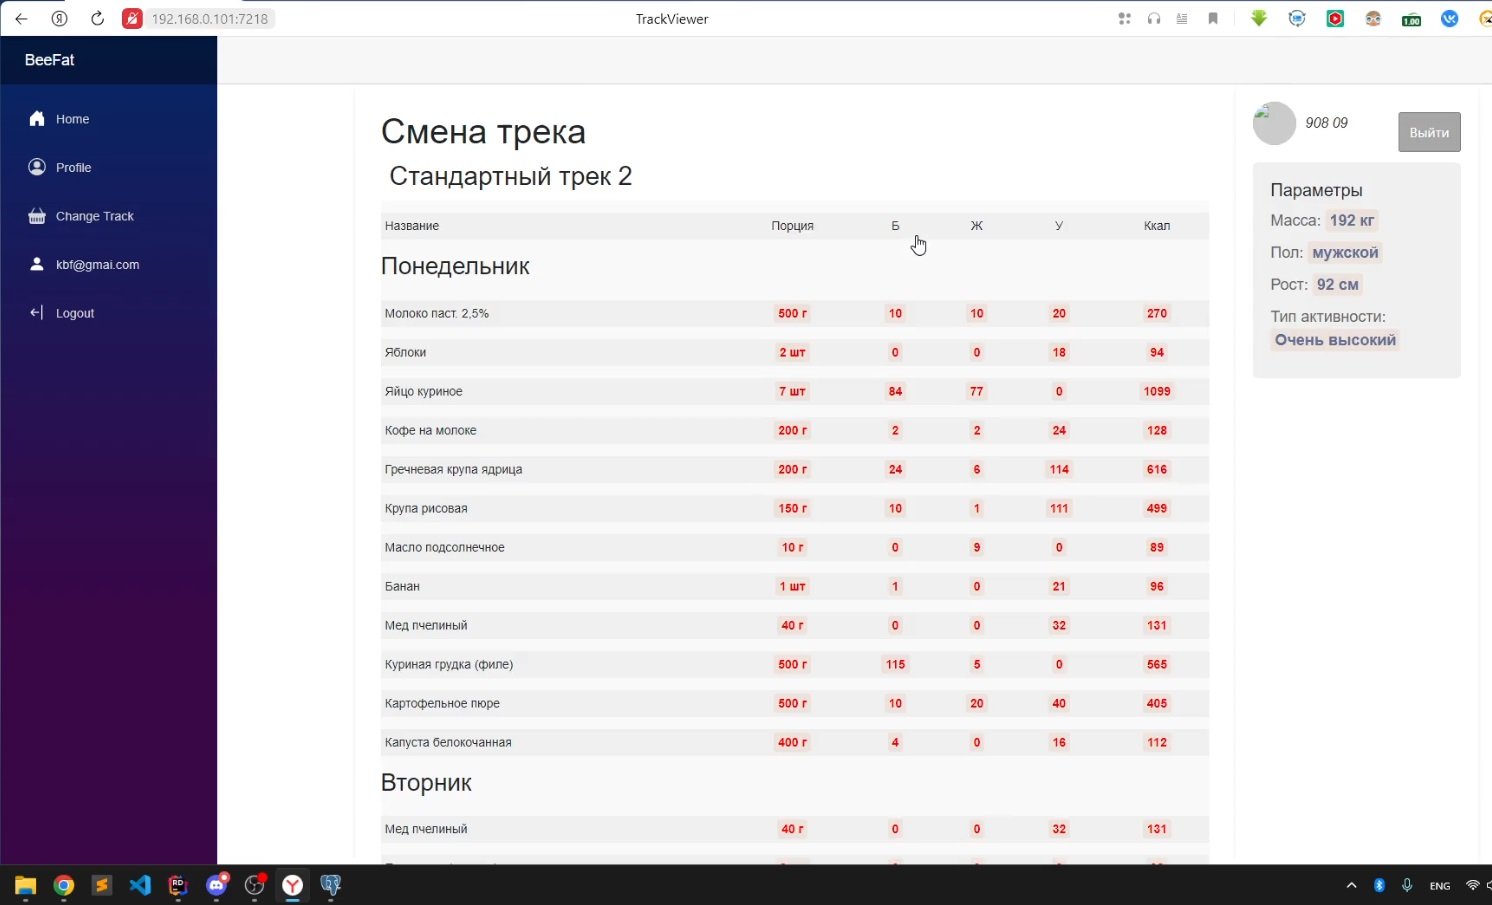
\includegraphics[width=10cm]{images/screenshot5.jpg}
}

\frame{ 
\frametitle{Скриншоты приложения}
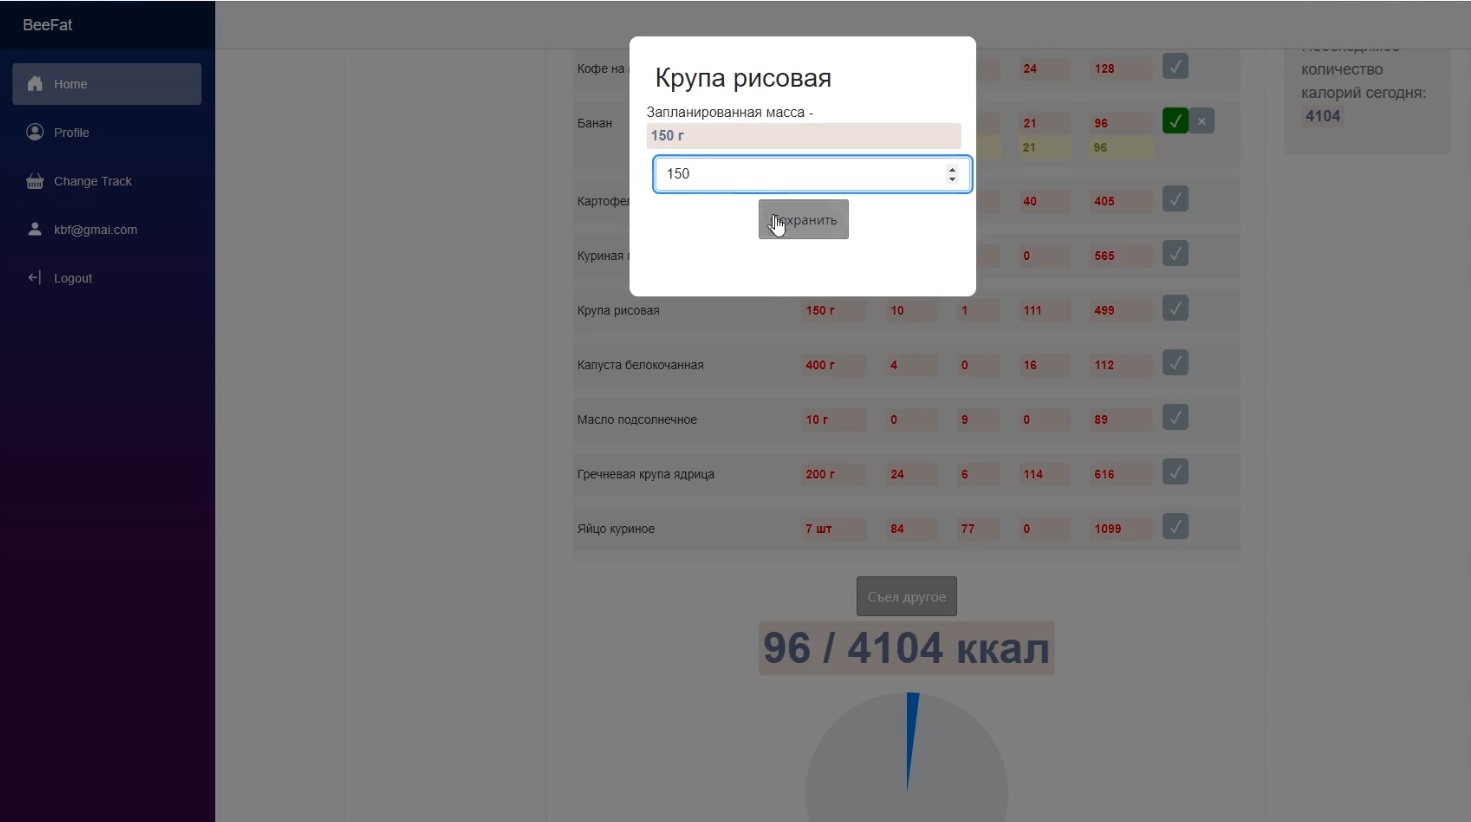
\includegraphics[width=10cm]{images/screenshot6.jpg}
}

\section{User-story} 
\frame{
\frametitle{User-story}
 
\begin{block}{User-story 1}
Я, как человек, который желает набрать массу, хочу иметь возможность планировать свое питание, чтобы достичь оптимальных результатов. 
\end{block}

\begin{block}{User-story 2}
Я, как человек, который желает набрать массу, хочу иметь возможность контролировать свое питание, чтобы быть в хорошей форме.
\end{block}
}


\section{Ключевая метрика} 
\frame{
\frametitle{Ключевая метрика}
\begin{block}{Ключевая метрика}
Время, которое пользователь тратил до нашего приложения и после.
\end{block}
Мы выбрали именно эту величину, потому что пользователю приходилось искать в интернете продукты, их калорийность, составлять себе план и т.д.
С нашим же приложением он очень сильно экономит время.
}

\frame{
\frametitle{Ключевая метрика}
Мы пообщались с тремя людьми, которые составляли план питания тремя способами:
\begin{itemize}
\item Блокнот + ручка
\item Таблицы (например excel)
\item Приложение "BeeFat"
\end{itemize}
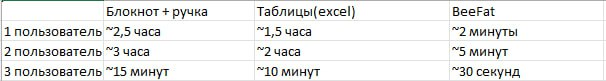
\includegraphics[width=10cm]{images/table.jpg}
}

\section{Отзывы}
\frame{
\frametitle{Отзывы}
\small
	1. "Идея клевая, но всегда не удобно вбивать то, что ты уже ел или тупо лень.... короче выбрать всегда прикольнее . но и получается у человека завязаны руки, когда он себе на день выбрал рацион? типо, а если я захочу банан.... но его нет в треке? какую-нибудь может быструю кнопку "компульсивный банан" добавить? и какую-нибудь статистику, как долго я не срывался на бананах? но это так, чисто у меня напрашиваются идеи как на чистом листе, только на белом сайте)))) это я к оформлению, но это не больших делов задача.
	
\small
Мне очень понравится трекер "заполняемости" когда ты уже съел норму или добил БЖУ, отображение очень нужно, я бы еще графически это как то выделила, типа, почти, почти почтиии, о да красавчик ты молодец все сожрал больше нельзя.

\small
Еще если именно по функциям, мне чет даже не к чему придраться, формат таблицы удобен, сбоку твой личный кабинет со всей инфой, идея треков мне зашла, обернуть бантиком надо!"
}

\frame{
\frametitle{Отзывы}

2. "Слишком всё просто сделано)
Хочется более интересного использования, каких-то дополнительных красивых и полезных приколюх
Непонятно, что делать, если случайно съел что-то не из плана, а может быть и неслучайно)
Нужна возможность добавлять к плану что-нибудь
В целом, сама тема заезженная, но вот идея с готовыми треками неплохая, надо сделать их побольше, поразнообразнее, возможно не только под набор массы
Следовал треку неделю, набрал 1 кг))"
}

\frame{
Вопросы?
}
\end{document}
